\def\year{2017}\relax
%File: formatting-instruction.tex
\documentclass[letterpaper]{article}
\usepackage{aaai17}
\usepackage{times}
\usepackage{helvet}
\usepackage{courier}
\usepackage{graphicx}
\usepackage{url}
\usepackage{color}
\usepackage{amsmath} 
\usepackage{verbatim}
\usepackage{flushend}
\newcommand{\tocheck}[1]{\textcolor{red}{#1}}

\newcommand{\papertitle}{Portable Navigation System with Adaptive Multimodal Interface for the Blind}

\frenchspacing
\setlength{\pdfpagewidth}{8.5in}
\setlength{\pdfpageheight}{11in}
\pdfinfo{
/Title (\papertitle)
/Author (Jacobus Lock, Grzegorz Cielniak, Nicola Bellotto)}
\setcounter{secnumdepth}{1}  
 \begin{document}
% The file aaai.sty is the style file for AAAI Press 
% proceedings, working notes, and technical reports.
%
\title{\papertitle}
\author{Jacobus Lock, Grzegorz Cielniak, Nicola Bellotto\\
Lincoln Centre for Autonomous Systems (L-CAS)\\
School of Computer Science, University of Lincoln\\
Lincoln LN6 7TS, United Kingdom\\
}
\maketitle

\begin{abstract}

Recent advances in mobile technology have the potential to radically change the quality of tools available for people with sensory impairments, in particular the blind and partially sighted. Nowadays almost every smart-phone and tablet is equipped with high-resolution cameras, typically used for photos, videos, games and virtual reality applications. Very little has been proposed to exploit these sensors for user localisation and navigation instead. To this end, the ``Active Vision with Human-in-the-Loop for the Visually Impaired'' (ActiVis) project aims to develop a novel electronic travel aid to tackle the ``last 10 yards problem'' and enable blind users to independently navigate in unknown environments, ultimately enhancing or replacing existing solutions such as guide dogs and white canes. This paper describes some of the project's key challenges, in particular with respect to the design of a user interface (UI) that translates visual information from the camera to guidance instructions for the blind person, taking into account the limitations introduced by visual impairment. In this paper we also propose a multimodal UI that caters to the needs of the visually impaired that exploits human-machine progressive co-adaptation to enhance the user's experience and improve navigation performance.

\end{abstract}

\section{Introduction}

The UK's Royal National Institute for the Blind (RNIB), a leading organisation in the area, has identified a number of challenges for the modern visually impaired (VI) person. These include the latter's ability to safely and independently use public transport and navigate in unfamiliar environments~\cite{rnib-objectives}. Recent technological advances allow for the creation of new solutions to address these challenges. GPS technology, for example, has become almost ubiquitous in the developed world. However, its accuracy is quite low -- typically a few meters --, is notoriously inaccurate in urban environments where satellite signals are blocked by high-rise buildings and have unreliable availability indoors. GPS-based devices are therefore unsuitable to identify and direct a user to high resolution targets such as a building's entrance or lift. To make a navigation system capable of successfully directing users to their desired locations will involve creating a system that can both localise the users within the world, i.e. by visually processing and understanding its surroundings, and communicate that information to them in a simple and effective way.

One promising avenue of research is making a hand-held mobile vision system to aid the navigation of the VI, extending concepts, such as sound-based navigation cues and progressive co-adaptation, as originally proposed in~\citeauthor{bellotto2013}, \citeyear{bellotto2013} and~\citeauthor{gallina2015}, \citeyear{gallina2015}. The main goal of the project ``Active-Vision with Human-in-the-Loop for the VI'' (ActiVis) can be thought of as solving a classic control problem where the process is the navigation system and the actuator is the VI user. The goal is to make a navigation system that can perceive its surroundings and convey safe navigation directions to the VI user in a way that minimises the control error (the difference between the user's desired and actual positions) as quickly as possible. To our knowledge, very little work has been done in this area, in particular with respect to control systems for humans~\cite{book-humancontrol}.

\begin{figure}
  \centering
  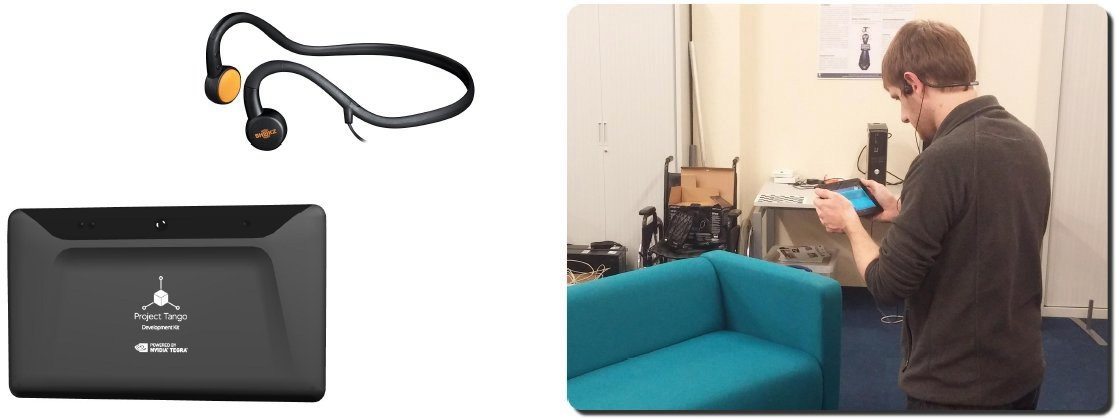
\includegraphics[width=0.8\columnwidth]{figures/fullset.jpg}
  \caption{The navigation system components and its application.\label{fig:fullset}}
\end{figure}

To overcome the barrier of user acceptability, ActiVis is based on a standard size tablet device, like the one illustrated in Fig.~\ref{fig:fullset} (the Google Project Tango). A key objective of the project is the development of an opportune user interface (UI) for this device, enabling communication between the navigation system and the human user. The UI should obviously take into account the user's visual impairment, but also the cognitive load which the user is exposed to when high-frequency sensor information is converted into navigation instructions to guide him/her. To this end, an important contribution of ActiVis will be the creation of a multimodal UI that uses audio and vibration cues to transmit navigational information to the VI person in the most effective way.    

Another objective of ActiVis is the implementation of a control system that exploits machine learning theory to adapt the UI's internal feedback parameters to match the user's level of skill and performance, taking into account the ``co-adaptation'' factor. The concept of human-machine co-adaptation is the simultaneous search for a global optimal by both the human and the machine. 

For any UI, there is a training period where a user familiarises himself with the different aspects of the UI where the user will eventually reach some optimal method to use and interpret the UI. However, since only the user is undergoing a training and adaptation period, this optimal may only be a local maxima. That is to say, if we implement a co-adaptation paradigm and allow the UI to adapt itself to the user as well, a global optimal may be reached that will allow the user to use the UI most effectively. 

Considering the user as the process adds an interesting aspect to the control problem: since controllers are typically designed for well-characterised electro-mechanical systems, while humans are known for the variability in their behaviour, it would be impossible to design a ``one-size-fits-all'' controller. A significant contribution of ActiVis to the active vision and human control fields will be a generic template controller that continuously monitors the user's performance and adapts the UI's internal parameters over time to match the human operator's navigation skill, thereby enhancing the complete system's (human operator included) navigation performance. On-line machine learning methods will be very suitable for this purpose. This project is therefore nicely placed at the intersection between the sensible UI design, machine learning and control theory fields. 

The remainder of the paper is organised as follows: Sec.~\ref{sec:literature} reviews some of the most relevant work, focusing in particular on navigation aids, UIs and adaptive systems for the VI; Sec.~\ref{sec:multimodal} presents some key aspects of the multimodal UI in ActiVis; Sec.~\ref{sec:adaptation} illustrates the co-adaptation concept applied to the proposed navigation system; finally, Sec.~\ref{sec:work} describes the current progress of the project and future steps to be taken towards achieving its objectives.

\section{Related Work}\label{sec:literature}

\subsection{Navigation Aids}

Producing a navigation and obstacle avoidance system for the VI is ActiVis's main goal. GPS technology, while undeniably useful, is not applicable here since it does not solve the so-called ``last 10 yards (or metres) problem'', where the VI user needs to be directed to a specific location 10m from him/her, e.g.\ the changing rooms in an unfamiliar department store. Different approaches have been investigated in literature; from so-called ``smart canes'' to RFID guidance and computer vision-based systems.

Early approaches to the problem of safe navigation for the VI involved augmenting the classic white cane with sensors such as ultrasound or laser sensors, to improve obstacle avoidance and warn the VI user of oncoming objects. The GuideCane system~\cite{ulrich1997}, for example, is a wheeled apparatus equipped with ultrasound sensors and motor encoders that the VI user pushes along the ground. The system is made in such a way that when an obstacle is detected, the wheels steer away to avoid the object and the VI person avoids the obstacle by adjusting his/her walking direction accordingly. The authors report successful tests with safe walking speeds of up to 1.5m/s. However, the system is clunky and clearly visible, which are two big obstacles to user acceptability and significant market penetration among the VI.

Using Radio Frequency Identification (RFID) technology for localisation and navigation has also been proposed. \citeauthor{willis2005} designed a system where a set of RFID tags encoded with spatial coordinates and location information are strategically placed around the environment~\cite{willis2005}. The VI users are then equipped with a cane or similar apparatus augmented with an RFID tag reader. Then, as the VI approaches an encoded tag, the RFID reader extracts the information which is then conveyed to the user. This allows the VI person to localise himself and learn about the descriptive features of the immediate environment. However, even though RFID tags and readers are relatively cheap and compact, installing a number of them across a location could be time consuming and costly since existing infrastructure might need to be adapted. Also, since the environment is typically dynamic and can change over time (for example a shop can close down), maintaining and updating such a system is also a concern.

More recently, with the rise in interest in computer vision, RGB-D sensors have become popular for navigation and object recognition tasks thanks to their relatively low cost, accuracy and their ability to output a scene's depth information. Various systems have been tested with varying degrees of success. One approach has allowed a computer to scan a scene for door-like shapes (e.g. bathroom doors, fire escapes, elevators, etc.) and extract contextual information from the door in the form of text or signage, which can then be conveyed to the VI user~\cite{tian2013b}. Other approaches involve using RGB-D information to build a 3D map of the environment and update it as the user traverses through it. In~\citeauthor{lee2015}, \citeyear{lee2015} the authors developed such a system, which is also capable of active collision avoidance, generating and continuously updating the shortest route to the user's desired destination. However, the person is directed along the route by a haptic feedback vest, which is a potential obstacle to usability and user acceptance.

The project described by~\citeauthor{chessa2016} created a system framework that carries out different computer vision tasks to assist a VI user~\cite{chessa2016}. These tasks include recognising faces it has seen before, so that it can tell the VI user if some known person is approaching, recognise and count cash amounts, and extract text from a scene to contextualise the environment. This is a promising framework, although only tested on videos recorded by a mobile phone. However it is a ``passive'' approach, in the sense that it does not actively guide the VI in performing a particular action, and where only a rudimentary UI has been implemented.

\subsection{Interfacing}

One of the main challenges in designing a navigation UI for the VI, besides easy ways to input desired destinations, is how to receive simple, unambiguous and accurate navigation instructions and environmental information conveyed in a way the VI user can understand and make sense of it. Feedback media such as vibration, spatialised sound, voice commands and image sonification have previously been considered in literature. 

\citeauthor{rogerio2014} performed a survey on the VIs' preferred feedback media~\cite{rogerio2014}. They found that the respondents overwhelmingly preferred systems which do not make the VI person stand out from the crowd and do not interfere with their daily functions. Furthermore, the respondents generally selected haptic and audio (including speech) feedback as their preferred feedback media, as opposed to electro-stimulation, for example. Interestingly, a haptic feedback-based navigation iPhone app (SpaceSense) received the most favourable reviews from the study's respondents. However, the study also highlighted that none of the systems they tested satisfied all of the VI's requirements.

With these results in mind, \citeauthor{frauenberger2003} created a so-called virtual audio reality (VAR) and implanted it with ``earcons'' (derived from the words ``ear'' and ``icons''), which represent pre-programmed notable features in the environment~\cite{frauenberger2003}. These earcons convey the features' position relative to the user with 3D spatialised sound. The authors report favourable results, but have not formally tested their system with VI users and they do not specify on how they plan to scale the system to be useful in unfamiliar environments where the position of features are unknown to the system. A similar system would be ``The Voice''~\cite{meijer2010}, which translates the image of a scene into a set of sinusoidal sound waves of varying pitch and volume.

On the front of user input,~\citeauthor{kane2011} found that if the VI user was limited to a typical touch screen interface, he/she showed a strong preference for gestures using screen corners, edges and multi-touch gestures, i.e.\ two or more fingers~\cite{kane2011}. They also found that gestures produced by the VI are larger, slower and display more variation in size than their sighted counterparts. Interestingly, when asked to invent their own gestures, the VI users came up with a technique not commonly seen in typical UIs designed for sighted users: they would touch the screen with a second finger to activate a specific mode and touch areas of the screen corresponding to QWERTY keys. Furthermore, \citeauthor{tian2013} found that the VI typically prefer to give input to the system through a QWERTY keyboard interface, rather than special icons~\cite{tian2013}. They also strongly prefer querying the system via voice commands for output rather than receiving a constant stream of feedback.

\begin{figure}
  \centering
  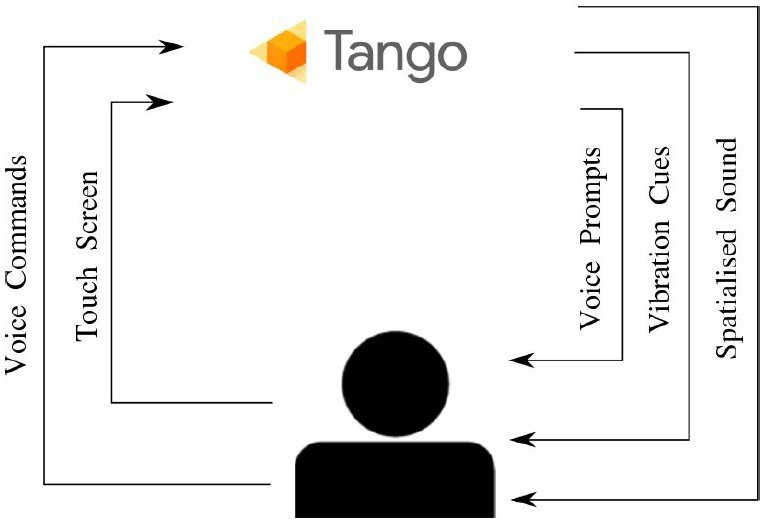
\includegraphics[width=0.8\columnwidth]{figures/multimodal.jpg}
  \caption{An illustration of the different feedback modes the UI employs.\label{fig:multimodal}}
\end{figure}

None of these factors are typically considered when designing an app interface for a normally sighted user, but as~\citeauthor{kane2011} and~\citeauthor{tian2013} show, they become very significant when the designer is trying to cater for non or partially-sighted users. Recent work by \citeauthor{bellotto2013}, upon which the current research is partly based, has looked at multimodal interfaces that can provide different sensory cues, audio- and vibration-based, to guide a VI person in pointing a mobile camera sensor towards landmarks and features of the environment useful for navigation (see Fig.~\ref{fig:multimodal})~\cite{bellotto2013}.

\subsection{Human-Machine Co-adaptation}\label{sec:co-adaptation}

Since task performance varies between different users, or even for the same user at different times, a mechanism for adapting to the user's skills and actual performance must be implemented to enable effective interaction between the VI user and the navigation system. However, most of the solutions proposed so far do not take these factors into account.

Several adaptive human-machine interfaces currently exist which are typically classified as \emph{human-centred} (or \emph{user-centred}) and \emph{goal-oriented}. The aim of the former is to create pleasant adaptive interfaces that maximize usability~\cite{Dixon2012}. In this case, the design focuses on user skills and expectations, developing interactive systems that prioritise their use, where human factors/ergonomics are applied together with usability knowledge and techniques~\cite{Jokela2003}.

The design of goal-oriented adaptive UIs, instead, focus on maximising the system's potential, assuming that the user is very skilled in performing the task. In this case, only well trained users can benefit from the adaptability of the interface. An example of goal-oriented interface is the one implemented in ``The Voice''~\cite{meijer2010}, where long training periods of the VI person are required to use the system effectively due to the amount of visual information translated by the latter to complex auditory signals for the user. More recently, a new ``progressive co-adaptation'' paradigm has been proposed by~\citeauthor{gallina2015}~\cite{gallina2015} that combines human-centred and goal-oriented advantages from which ActiVis could benefit to overcome the limitations of previous VI interfaces.

\section{Multimodal Interface}\label{sec:multimodal}

\begin{figure}
  \centering
  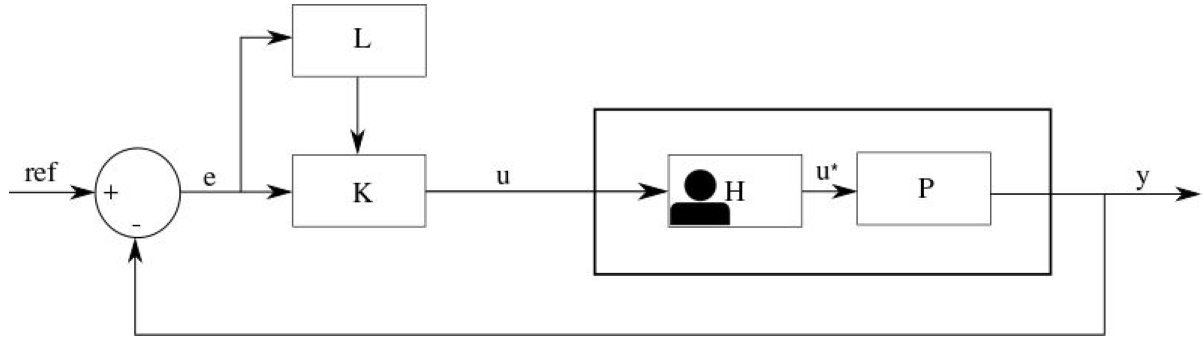
\includegraphics[width=0.8\columnwidth]{figures/loop.jpg}
  \caption{Progressive co-adaptation with human-in-the-loop.\label{fig:loop}}
\end{figure}

A key aspect that differentiates ActiVis from most of the active vision systems in the literature~\cite{Rivlin2000} is the human-in-the-loop aspect: That is the fact that the process to be controlled is not an electro-mechanical actuator panning and tilting the camera, but the hand, arm and body of the user holding it. Consequently, the control signal, $u$ (see Fig.~\ref{fig:loop}), that instructs the movement of the human actuator is not a particular current or voltage, but a sensory input (audio-tactile interface) for the VI user. 

In ActiVis, the multimodal navigation system is based on an Android app developed specifically for Google's Project Tango device (see Fig.~\ref{fig:fullset}), developed with the standard Android and Tango SDKs. The latter gives access to Project Tango's three core capabilities: motion tracking, depth perception and area learning. These technologies allow the Tango to accurately localise itself and perceive its surroundings. The depth perception and area learning capabilities are of particular interest to this project. It is also worth noting that the Tango SDK's are currently closed-source and developed and maintained by Google themselves and we therefore have little control over how the Tango performs its image processing tasks. 

Thanks to the Tango's localisation capabilities, getting from point A to B is relatively simple; the real challenge lies in directing the VI user toward point B along a route as quickly and safely as possible. Building a navigation app with a UI optimised for the visually impaired is obviously crucial here. 

The navigation system in its current form guides the user toward a particular target using voice commands and spatialised sound, while vibration is used for obstacle avoidance. The spatial sound has 3 parameters that convey the target's position relative to where the user is pointing the Tango's camera and its current position: the pitch (elevation angle to the target), gain (absolute distance to the target) and 3D panning (whether the target is to the left or right of the user). The solution is partially based on previous work in multimodal UIs for the blind~\cite{bellotto2013}, extending it here to take into account the enhanced perception capabilities of the Tango device.

The multimodal UI also enables the implementation of a co-adaptive module, responsible to learn the behaviour of the user over time and adapt the navigation system's feedback parameters to improve performance, i.e.\ get the user to his desired location quicker by conveying its navigation instructions more effectively. Examples include learning the frequency of the user's voice feedback requests, the intensity of the vibrations required and the user's most common location requests. The following section discusses more in detail the approach that will be used to implement this module in ActiVis.

\section{Progressive Co-adaptation}\label{sec:adaptation}

Most of the existing co-adaptive techniques assume that there is a well-defined link between the optimal UI, $\Psi$, and the user's skill, $\Phi$, to accomplish a task, so in theory it is possible to associate a particular interface or UI parameter to pre-determined (or static) skill levels. However, in many cases, the UI should also adapt dynamically to possible changes in the user's level of skill over time in order to escape a potential local maxima and maximise the overall performance. Therefore, co-adaptive approaches have been proposed that take into account time, $t$, as  key parameter of the UI, paying attention to the actual adaptation rate of the UI, $\frac{d\Psi}{dt}$, to guarantee the stability of the entire system~\cite{Merel2013}.

Recent work extended this further by considering not only time and user skills, but their rates of change, $\frac{d\Phi}{dt}$ as well~\cite{gallina2015}. The idea here is that by observing the rate at which the user's skill vary over time, it is possible to detect when a plateau is reached -- i.e. the user is not able to improve task performance any further. The UI could be regulated then by variations $\frac{d\Phi}{dt}$ to implement a progressive co-adaptation system, where the user-navigation system achieves gradual, but steady improvements in task performance that goes beyond local maxima toward a global maxima.

In ActiVis, the latter form of co-adaptation will be implemented in a parameterised UI by following the goal-orientated approach discussed in Sec.~\ref{sec:co-adaptation}. These parameters include variable amplitudes and frequencies of voice instructions, sounds and vibrations, and the measurable user skills are those related to his/her capability to move and point the mobile device as instructed by the navigation system. The adaptive module, $L$, in Fig.~\ref{fig:loop} will therefore include a control law that is a function of the user's skills (measured, for example, as the average error between the device's actual and desired positions) and their rates of change.

Since every controller will eventually differ from one another depending on the user and his level of skills and performance, we opt to follow a template design route with regards to the adaptable controller. This template will act as an optimal starting point which the adaptation law can use to eventually reach a global maxima. 

The adaptable controller will be designed using concepts from the fields of on-line machine learning. The entire process may even be considered a partially observable Markovian decision process (POMDP), where the optimal solution (i.e.\ the the most suitable UI for any user) will be determined given a set of partially observable states of the user and the world. POMDP's have already successfully been implemented for autonomous robot navigation and model determination~\cite{ross2008bayesian}. Our approach will be similar, but it will have to be adapted for a more complex process model with access to fewer states. 

\section{Current and Future Work}\label{sec:work}

The current implementation of the ActiVis system is an Android app based on a Tango device and an AfterShokz Sportz 3 bone-conducting headset (see Fig.~\ref{fig:fullset}). Through the latter, the user can listen to sounds and voice instructions generated by the Tango without affecting normal hearing. Along with a set of sensors commonly found in modern smart phones (vibration, 3-axis gyroscope and accelerometer, touch screen, GPS, etc.), the Tango comes equipped with a set of RGB-D camera's that allows it to perceive its environment in 3D.

Developing a navigation app on a mature, widely used and well-supported platform like Android provides a multitude of input/output options. For example, speech recognition and gesture support are built in by default. Furthermore, Android's native code support makes it easy to integrate C/C++ libraries, such as OpenCV (for computer vision tasks), OpenAL and OpenSL (sound generating libraries with sound spatialisation support), into an app, presenting an opportunity to create a unique, interesting and rich UI for a VI user. Adding a peripheral device (e.g. via USB) to produce more diverse vibrations can also be considered.

The app is mostly written in Java using the standard Android SDK with extra Tango libraries and support and uses the OpenAL native library to generate spatial sound signals. The system is capable of recording various parameters in real-time, including 3D position and rotation of the device. The Android SDK also allows the streaming, recording and visualisation of these parameters in real-time using a PC connected to the Tango's WiFi network.

\subsection{Virtual Cane}

The app's current implementation is inspired by the white cane widely used by the VI: By using the depth data from the Tango's RGB-D sensor, the system can tell the user when an obstacle is approaching by using the Tango's built-in vibration interface. The obstacle's distance can also communicated by adjusting the vibration intensity.  

Furthermore, a navigation feature is built into the Virtual Cane app, which allows the user to program a destination. The user is guided towards the target using the multimodal UI described in Sec.~\ref{sec:multimodal}, which includes voice commands and spatialised sounds.

For testing purposes, the system takes advantage of the Tango's place recognition capabilities, which allow for more robust and reliable position tracking over longer distances. It also provides a platform for testing the multimodal feedback with VI users and record their performances in navigation tasks for further studies in human-machine co-adaptation. The Virtual Cane app also provides a good starting point to implement the co-adaptive module. 

\subsection{Planned Experiments}

To create the co-adaptation module, it is necessary to know how the different feedback modes affect each individual user's navigation performance, e.g. whether more intense vibration results in more effective obstacle avoidance or vice-versa. A set of experiments have been planned to determine how the four feedback parameters of the multimodal UI affect user performance. These parameters are the pitch gain rate, the volume gain rate, vibration period and voice command frequency. The sound panning is controlled by a separate library so it is not included as a variable in these tests. 

The first set of experiments is to have the user traverse through an obstacle course on a 2D plane where the exit of the course will be the final target. Since the latter is at a fixed height, the pitch variable is not considered here, which simplifies the experiment. Only the vibration, voice commands and volume gain are used for feedback. 

A separate set of tests will be conducted to determine the effect of the pitch and spatial sound, where the user will be directed to point the Tango to look at virtual targets floating at different levels and distances to the user. Here the vibration parameter will be eliminated and only the voice commands, pitch and volume gain will be used as feedback parameters. 

A final set of tests will be conducted with all of the feedback parameters enabled. This set of tests will be more large-scale than the previous ones and will only be carried out when we have finished processing the data and have the results ready from the previous sets of tests. 

\subsection{Next Steps}

After the test data has been analysed to have a better understanding of how the different feedback parameters affect a user's navigation performance, the project will continue to create and integrate an autonomous co-adaptation module into the Tango. This will be responsible for monitoring a user's navigation performance and adapt the feedback parameters in real-time to improve such performance.

\section*{Acknowledgment}

This research is partially funded by a Google Faculty Research Award (Winter 2015). 

\bibliographystyle{aaai}
\bibliography{aaai17google}

\end{document}
